\section*{Math 202A - HW11 - Dan Davison - \texttt{ddavison@berkeley.edu}}

\begin{mdframed}
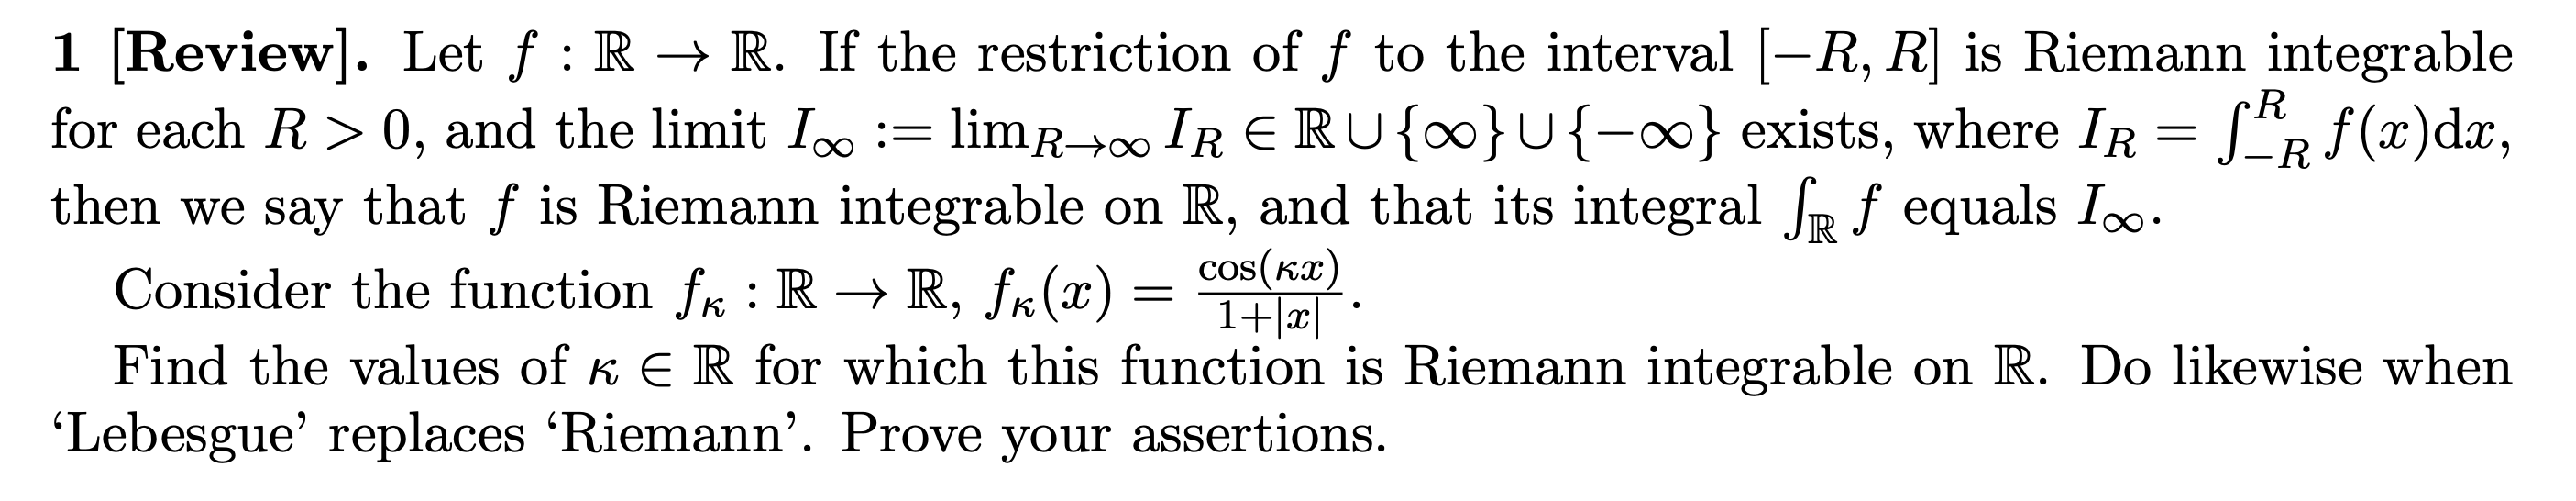
\includegraphics[width=400pt]{img/analysis--berkeley-202a-hw11-8650.png}
\end{mdframed}

\begin{lemma}[Dirichlet's test for improper integrals]
  Let $I = \int_a^\infty f(x) g(x) \dx$ where $\int$ denotes the Riemann integral. Then $I$ converges if all
  the following are true
  \begin{enumerate}
  \item $f$ is continuous on $[a, \infty]$
  \item $\int_a^x f(t) \dt$ is bounded on $[a, \infty]$
  \item $g$ is differentiable on $[a, \infty]$ with $g' \leq 0$ and $\lim_{x\to\infty} g(x) = 0$.
  \end{enumerate}
\end{lemma}

\begin{proof}
  Note that $f_\kappa$ is an even function, therefore (hint from @ankit in
  Slack) $\int_{-R}^R f_{\kappa}(x) \dx = 2\int_{0}^R f_\kappa(x)$ and
  therefore $I_\infty = \frac{1}{2}\int_0^\infty f_{\kappa}(x) \dx$, if this limit (in the upper bound of the
  integral) exists.

  We now (hint from Piazza) invoke Dirichlet's test with $a = 0$, $g(x) = 1/(1 + x)$,
  and $f(x) = \cos(\kappa x)$, where these variable names refer to the statement in the lemma. We see that $f$
  is continuous on $[0, \infty]$ as required; we see that $\int_0^x f_{\kappa}(t) \dt = \sin(\kappa t)$ is
  bounded on $[0, \infty]$; and we see that $g$ is differentiable on $[0, \infty]$ with $g'(x) = -1/(1 + x)^2$
  and that $g(x) \to 0$ as $x \to \infty$. Therefore we conclude that $\int_0^\infty f_{\kappa}(x) \dx$
  converges and therefore that $f_{\kappa}$ is Riemann integrable for all $\kappa$.

  By definition, $f_{\kappa}$ is Lebesgue integrable if $\int_{-\infty}^\infty |f_{\kappa}| < \infty$.
  Since $|f_{\kappa}|$ is even and non-negative, $f_{\kappa}$ is Lebesgue integrable if and only
  if $\int_{0}^\infty |f_{\kappa}| < \infty$.

  Note that (by considering the graphs of $|\cos(\kappa x)|$ and $1/(1 + x)$)
  \begin{align*}
    \int_{0}^\infty |f_{\kappa}|
    = \int_0^\infty \frac{|\cos(\kappa x)|}{1 + x}
    > \(\int_0^{2\pi}|\cos(\kappa x)|\) \sum_{n=1}^\infty \frac{1}{1 + 2n\pi}.
  \end{align*}
  Clearly $\int_0^{2\pi}|\cos(\kappa x)| > 0$. But $\sum_{n=1}^\infty \frac{1}{1 + 2n\pi}$ is a divergent
  series, therefore $f_{\kappa}$ is not Lebesgue integrable for any value of $\kappa$.
\end{proof}


\begin{mdframed}
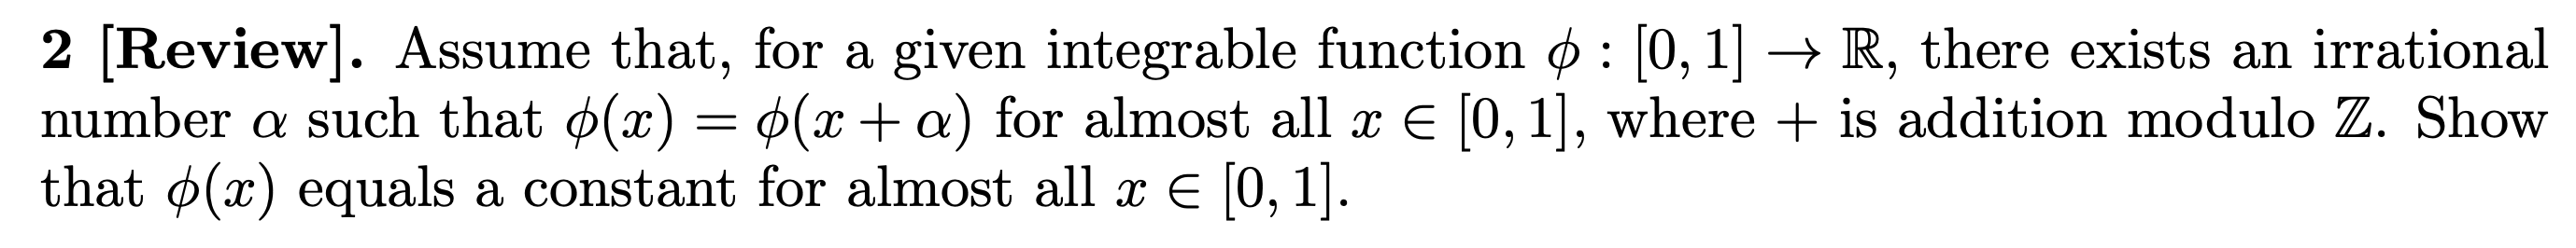
\includegraphics[width=400pt]{img/analysis--berkeley-202a-hw11-b6a3.png}
\end{mdframed}

\begin{proof}
  We will prove this by contradiction. Let $P$ be the proposition
  \begin{quote}
    There exists $y \in \R$ such that $m(\{x \in [0, 1] ~:~ \phi(x) < y\}) > 0$ and $m(\{x \in [0, 1] ~:~ \phi(x) > y\}) > 0$.
  \end{quote}
  Since $\phi$ is integrable, it is measurable, and therefore these preimages are measurable sets.

  The statement
  \begin{quote}
    ​$\phi(x)$ equals a constant a.e.
  \end{quote}
  is false if and only if $P$ is true. Therefore we suppose, for a contradiction, that $P$ is true.

  Let $\tau: [0, 1) \to [0, 1)$ be the map defined by $x \mapsto x + \alpha \mod \Z$, and let $y \in \R$ be a
  value satisfying $P$, such that $A = \{x \in [0, 1] ~:~ \phi(x) < y\}$
  and $B = \{x \in [0, 1] ~:~ \phi(x) > y\}$ both have positive measure.

  But recall from HW6 Q6 that $\mu(\bigcup_{n=0}^\infty \tau^n(E)) = 1$ for every set $E \subseteq [0, 1]$,
  where $\tau^n(E)$ is the image of $E$ under the $n$-th iterate of $\tau$.

  Therefore $\mu(\bigcup_{n=0}^\infty \tau^n(A)) = 1$. But we have $\phi(x) = \phi(x + \alpha)$ a.e. therefore
  (should justify this better) $m(\{x \in \bigcup_{n=0}^\infty \tau^n(A) ~:~ \phi(x) < y\}) = 1$.

  Similarly $\mu(\bigcup_{n=0}^\infty \tau^n(B)) = 1$ and $m(\{x \in \bigcup_{n=0}^\infty \tau^n(A) ~:~ \phi(x) > y\}) = 1$.

  But this is a contradiction, since simultaneously have $\phi(x) < y$ a.e. and $\phi(x) > y$ a.e., which
  violates countable additivity of $m$.
\end{proof}

% The problem with the thoughts below, I think, is that the function $\phi$ being described is not measurable.

% This is true because the orbit of the map $x \mapsto x + a$ is dense in $[0, 1]$. We basically just need to show that.

% We must show that $\phi(x)$ equals a constant for almost all $x$.

% Why should that be? Why, for example, can't each orbit have its own constant value?


% \begin{proof}
%   Let $\tau: [0, 1) \to [0, 1)$ be the map defined by $x \mapsto x + \alpha \mod \Z$, and for $x \in [0, 1)$
%   define the sequence $(r_n(x)) = x, \tau(x), \tau^2(x), \ldots$, and
%   let $\orb(x) := \big\{r_n(x) ~:~ n \in \N\big\}$ be the orbit of $x$ under $\tau$. Recall from HW2 and HW6
%   that for each $x \in [0, 1)$ the sequence $(r_n(x))$ is non-repeating, the corresponding orbit $\orb(x)$ is
%   dense in $[0, 1]$, and each orbit is disjoint from every other orbit. Thus each orbit is a countable set and
%   there are uncountably many distinct orbits.

%   We have that the set of points $x$ at which $\phi(\tau(x)) = \phi(x)$ has measure $1$. Therefore we have the
%   following qualitative picture: there are uncountably many disjoint orbits and each orbit is associated with a
%   sequence $\phi(x), \phi(\tau(x)), \phi(\tau^2(x)), \ldots$. The set of points at which this sequence changes
%   value has measure $0$.

%   We must use the fact that $\phi$ is integrable to show that $\phi$ is constant a.e.

%   Let $\eps > 0$ and let $g: [0, 1] \to \R$ be a continuous function such that
%   \begin{align*}
%     \int |g - \phi| < \eps.
%   \end{align*}






%   Let $\eps > 0$. According to Lusin's theorem there exists a closed set $F \subseteq [0, 1]$
%   with $m(F) > 1- \eps$ such that $\phi|_F$ is continuous. So let $F \subseteq [0, 1]$ be such that $m(F) = 1$
%   and $\phi|_F$ is continuous.

%   Note that $F$ is uncountable and therefore it contains points from uncountably many orbits.


%   Probabilistic view:

%   - Pick $x$. It is a member of some orbit and has some value $\phi(x)$. We have $Pr(\phi(x + \alpha) = \phi(x)) = 1$.

%   - Suppose the claim is not true. Then there exist $c$ and $d$ such that $m(\phi = c) = p_c > 0$ and $m(\phi = d) = p_d > 0$.

%   - Pick $x$. With probability $p_c$ we have $\phi(x) = c$ and also $\phi(x + \alpha) = c$.










%   Why might $\phi$ be constant a.e.?

%   - Each orbit is countable, so if one orbit is constant, that's just a measure zero set.

%   - Similarly, if every orbit is constant, but they all have different values that's not constant a.e.

%   - What we need to show is something more like that all orbits ``start​'' with the same value

% \end{proof}

\begin{mdframed}
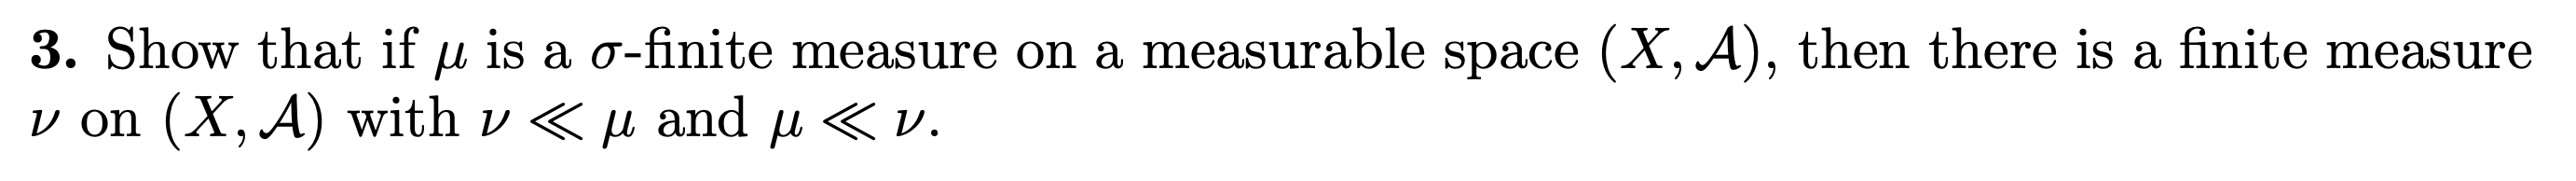
\includegraphics[width=400pt]{img/analysis--berkeley-202a-hw11-3704.png}
\end{mdframed}

\begin{proof}
  Since $\mu$ is $\sigma$-finite we can write $X$ as a countable disjoint union $X = \bigcup_{i=1}^\infty X_i$
  with $\mu(X_i) < \infty$ for all $i$.

  Let $\nu$ be a set function such that for every $A \in \mc A$
  \begin{align*}
    \nu(A) = \sum_{i=1}^\infty 2^{-i} \frac{\mu(A \cap X_i)}{\mu(X_i)}.
  \end{align*}
  We claim that $\nu$ is a measure. We have $\nu(\emptyset) = 0$. Let $A_1, A_2, \ldots \in \mc A$ be pairwise
  disjoint. We see that $\nu$ is countable additive since
  \begin{align*}
    \nu\(\bigcup_{j=1}^\infty A_j\)
    &= \sum_{i=1}^\infty 2^{-i} \frac{\mu\(\(\bigcup_{j=1}^\infty A_j\) \cap X_i\)}{\mu(X_i)} \\
    &= \sum_{i=1}^\infty 2^{-i} \frac{\mu\(\bigcup_{j=1}^\infty \(A_j \cap X_i\)\)}{\mu(X_i)} \\
    &= \sum_{i=1}^\infty 2^{-i} \sum_{j=1}^\infty\frac{\mu\(A_j \cap X_i\)}{\mu(X_i)} \\
    &= \sum_{j=1}^\infty \sum_{i=1}^\infty 2^{-i}\frac{\mu\(A_j \cap X_i\)}{\mu(X_i)} \\
    &= \sum_{j=1}^\infty \nu(A_j).
  \end{align*}
  Therefore $\nu$ is a measure. Furthermore $\nu$ is finite since $\nu(X) = \sum_{i=1}^\infty 2^{-i} = 1$.

  If $A \in \mc A$ and $\mu(A) = 0$ then
  \begin{align*}
    0 \leq \nu(A)
    = \sum_{i=1}^\infty 2^{-i} \frac{\mu(A \cap X_i)}{\mu(X_i)}
    < \sum_{i=1}^\infty 2^{-i} \frac{\mu(A)}{\mu(X_i)}
    = 0,
  \end{align*}
  hence $\nu \ll \mu$. Finally, if $A \in \mc A$ and $\nu(A) = 0$ then $\mu(A \cap X_i) = 0$ for all $i$,
  therefore $\mu(A) = \sum_{i=1}^\infty \mu(A \cap X_i) = 0$, since the $X_i$ partition $X$.
\end{proof}



\begin{mdframed}
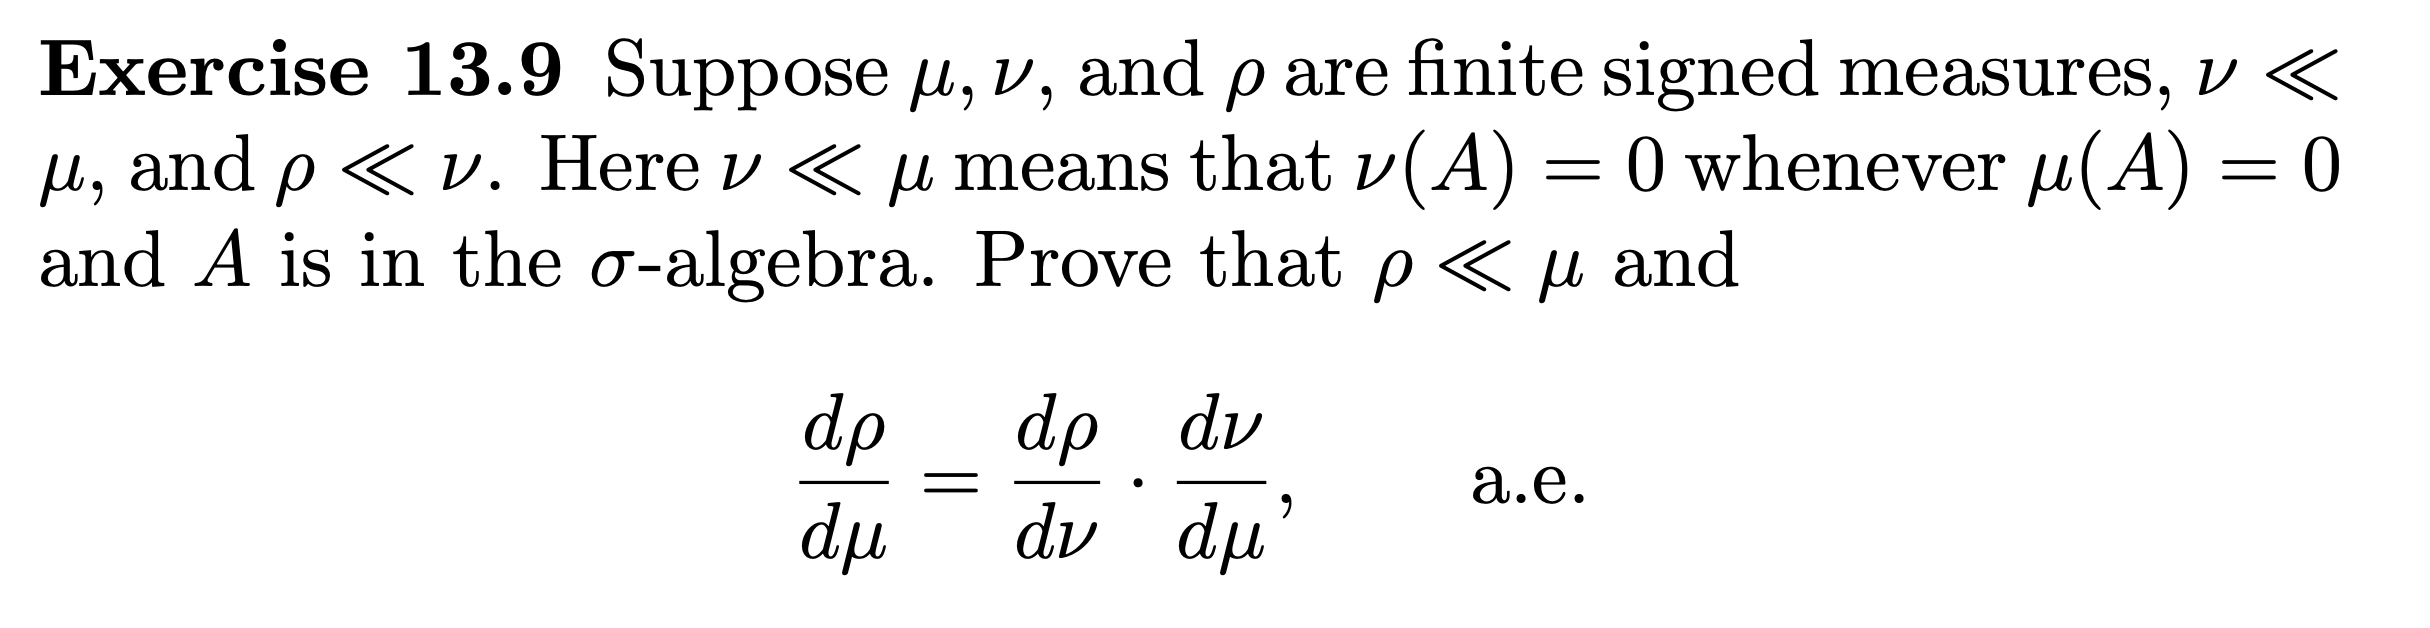
\includegraphics[width=400pt]{img/analysis--berkeley-202a-hw11-f2c0.png}
\end{mdframed}


\begin{claim*}
  $\rho \ll \mu$
\end{claim*}
\begin{proof}
  We must show that $\rho(A) = 0$ whenever $\mu(A) = 0$ and $A$ is in the $\sigma$-algebra.

  Let $A$ be in the $\sigma$-algebra such that $\mu(A) = 0$. Then $\nu(A) = 0$, since $\nu \ll \mu$.
  Therefore $\rho(A) = 0$, since $\rho \ll \nu$.
\end{proof}

\begin{claim*}
  \begin{align*}
    \frac{\d\rho}{\d\mu} = \frac{\d\rho}{\d\nu}\frac{\d\nu}{\d\mu} \ae
  \end{align*}
\end{claim*}

\begin{proof}
  By definition, $\frac{\d\rho}{\d\mu}$ is a function such that for any measurable set $E$
  \begin{align*}
    \rho(E) = \int_E \frac{\d\rho}{\d\mu} \d\mu.
  \end{align*}
  We will first show that the function $\frac{\d\rho}{\d\nu}\frac{\d\nu}{\d\mu}$ also serves as a derivative
  of $\rho$ with respect to $\mu$, i.e. that for any measurable set $E$
  \begin{align*}
    \rho(E) = \int_E \frac{\d\rho}{\d\nu}\frac{\d\nu}{\d\mu} \d\mu.
  \end{align*}
  Let $E$ be a measurable set.

  Write $f = \frac{\d\rho}{\d\nu}$ and let $f_n$ be a sequence of increasing simple functions converging
  pointwise to $f$. Let $F$ be a measurable set and note that
  \begin{align*}
    \int_E \ind_F \d\nu
    = \nu(E \cap F)
    = \int_{E \cap F} \frac{\d\nu}{\d\mu} \d\mu
    = \int_E \ind_F \frac{\d\nu}{\d\mu} \d\mu.
  \end{align*}
  By linearity of the integral this result applies to the simple functions $f_n$ and we have
  \begin{align*}
    \int_E f_n \d\nu = \int_{E} f_n \frac{\d\nu}{\d\mu}\d\mu,
  \end{align*}
  and on taking the limit $n \to \infty$ inside the integral (\red{I think I should be using MCT somewhere, could you tell me where?})
  \begin{align*}
    \int_E f \d\nu = \int_{E} f \frac{\d\nu}{\d\mu}\d\mu.
  \end{align*}
  Substituting its definition $\frac{\d\rho}{\d\nu}$ in place of the symbol $f$ we have
  \begin{align*}
    \int_E \frac{\d\rho}{\d\nu} \d\nu
    = \rho(E)
    = \int_E \frac{\d\rho}{\d\mu} \d\mu
    = \int_{E} \frac{\d\rho}{\d\nu} \frac{\d\nu}{\d\mu}\d\mu.
  \end{align*}

  Therefore
  \begin{align*}
    \int_E \frac{\d\rho}{\d\mu}  - \frac{\d\rho}{\d\nu}\frac{\d\nu}{\d\mu} \d\mu = 0,
  \end{align*}
  and therefore by Bass proposition 8.2
  \begin{align*}
    \frac{\d\rho}{\d\mu} = \frac{\d\rho}{\d\nu}\frac{\d\nu}{\d\mu} \ae
  \end{align*}
\end{proof}

\begin{mdframed}
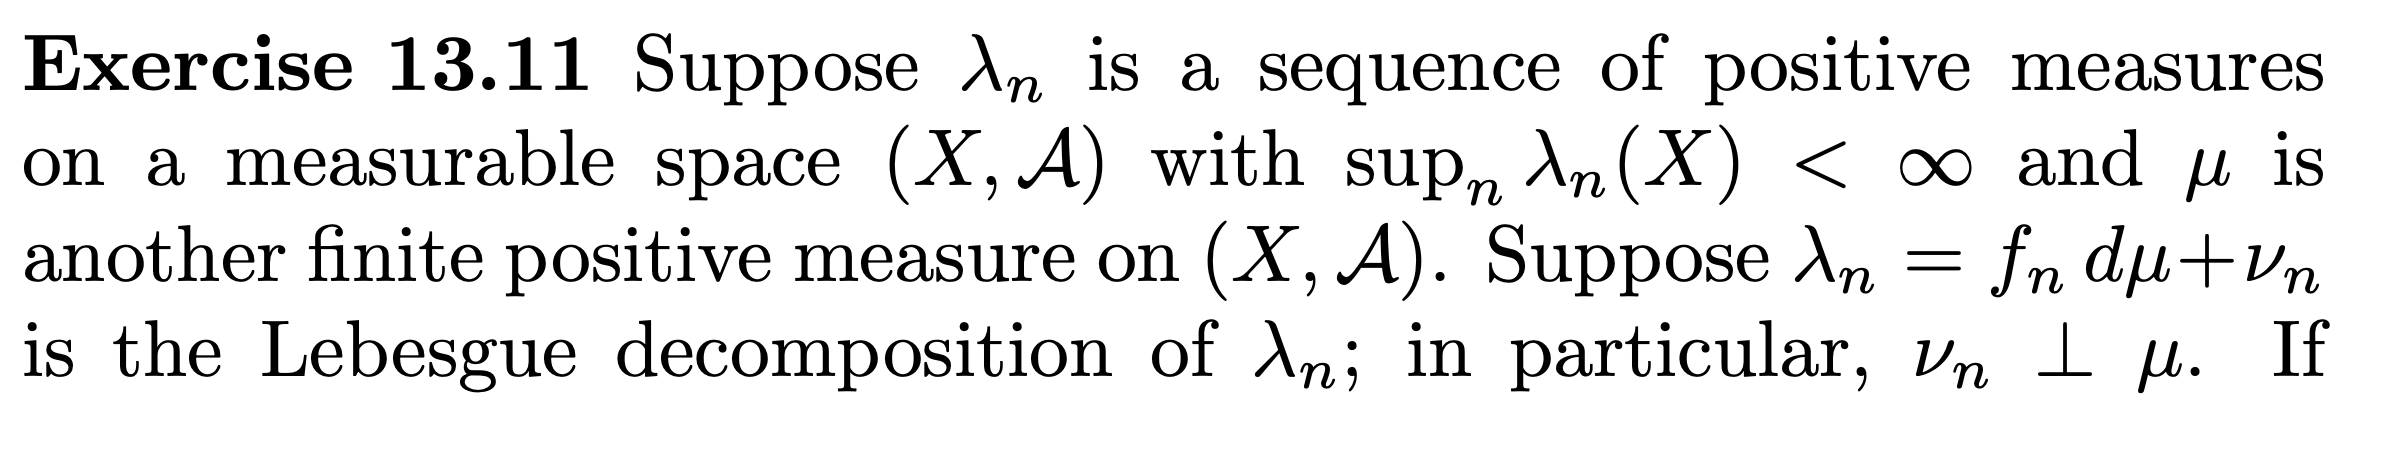
\includegraphics[width=400pt]{img/analysis--berkeley-202a-hw11-c5a4.png}
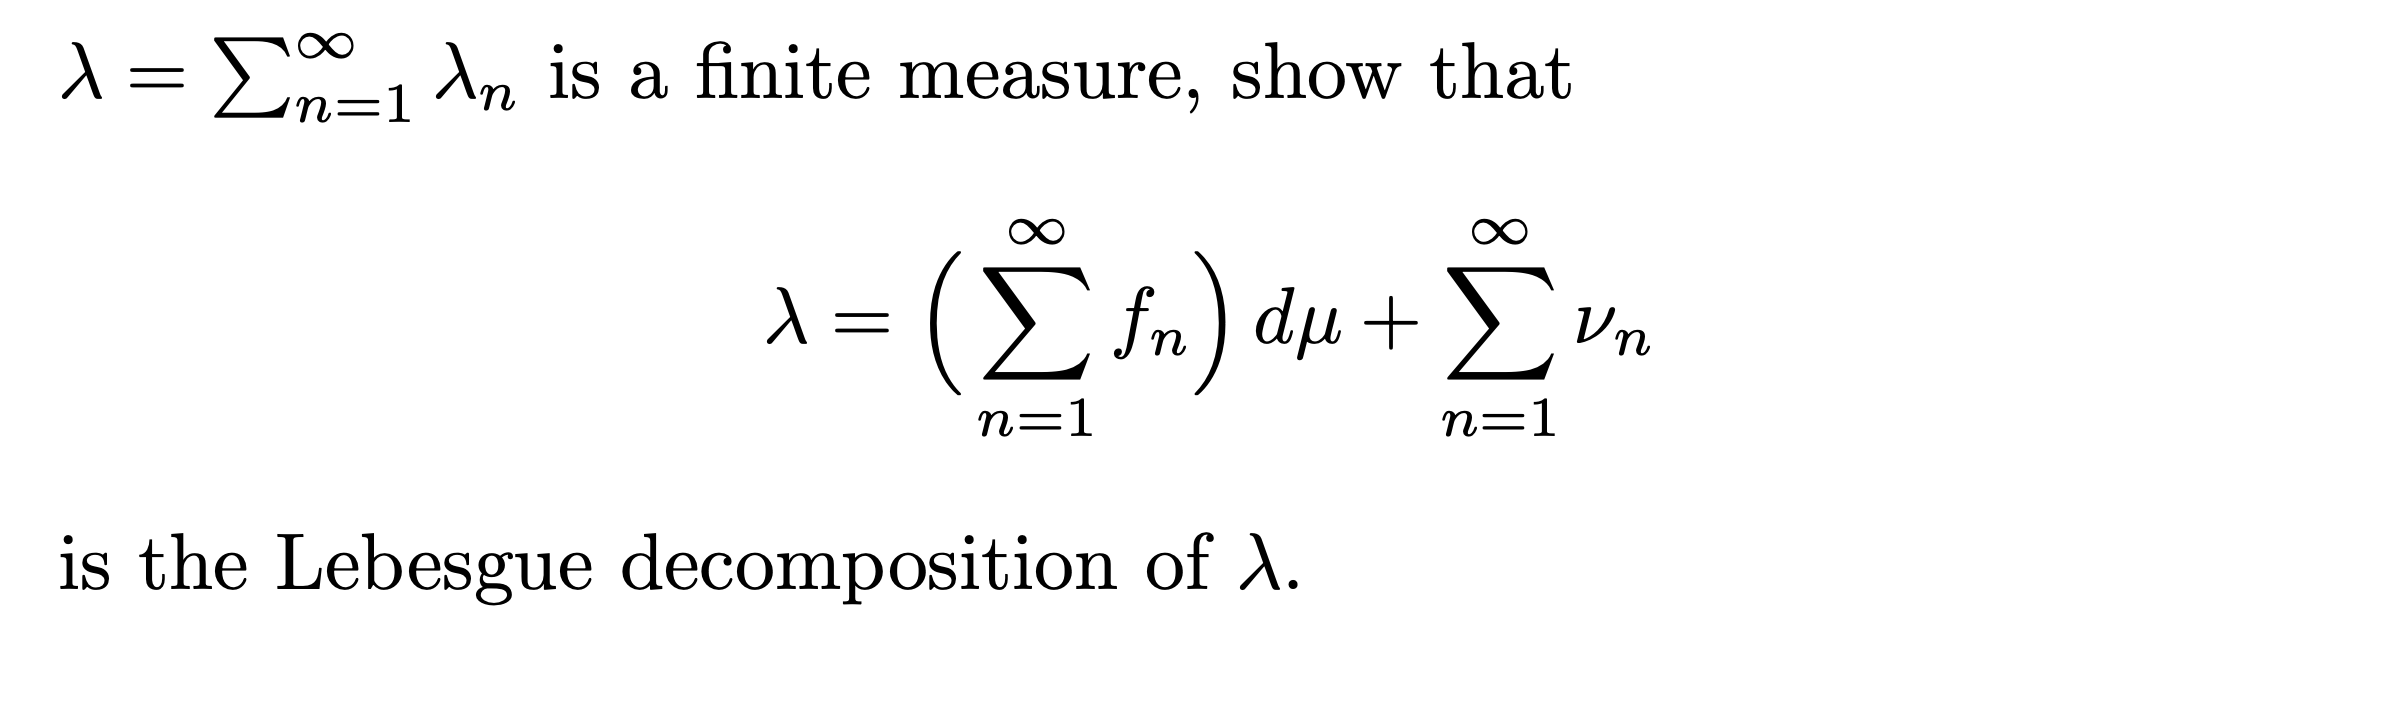
\includegraphics[width=400pt]{img/analysis--berkeley-202a-hw11-3974.png}
\end{mdframed}